\cotefile{147}

\scanpage{80}
\mspage{39}
\[
\tag{\unsure{102|107}}
\diagram{\begin{tikzcd}[ampersand replacement=\&, column sep=large,row sep=large]
\& \Pi M^*_{\underline G,\underline G'} \arrow[r] \arrow[d] \& \Pi M_{G'} \\
\Pi(M_{\underline G}\deleted{,\unsure{\Gamma^!_{\underline G,\underline G'}}}) \arrow[r,"\approx"{name=equiv80}] \& \Pi M_{G,G'} \\
\& \begin{gathered}\text{ceci est une}\\\text{équivalence de}\\\text{groupoïdes}\end{gathered}
\arrow[from=equiv80,to=3-2,bend right=45]
\end{tikzcd}}
\]
qu'on va réécrire comme
\[
\tag{103}
\diagram{\begin{tikzcd}[ampersand replacement=\&, column sep=large,row sep=large]
\Pi M^*_{\underline G,\underline G'} \arrow[r,"\unsure{\gamma_{\underline G,\underline G'}|\psi_{\underline G,\underline G'}}"] \arrow[d,"\varphi_{G,G'}"] \& \Pi M_{G'} \\
\Pi(M_G,\deleted{\unsure{\Gamma^!_{\underline G,\underline G'}}})
\end{tikzcd}}
\]
\margin{``diagramme de générisation pour les groupoïdes fondamentaux pour le quotient de $\underline G\to\underline G'$''}
\deleted{\unsure{mais} pour la suite, il sera plus commode d'écrire $\Pi M_{G,G'}$ \unsure{au} lieu de $\Pi(M_G,\unsure{\Gamma^!_{\underline G,\underline G'}})$}

L'hom des groupoïdes $\varphi_{G,G'}$ propriétés de \deleted{\unsure{la}} l'hom sur les $\pi_1$ dans une fibration de base $(M_G\deleted{,\unsure{\Gamma_{\underline G,\underline G'}}\inserted{\text{op. de }\Gamma^!_{G,G'}}})$, \deleted{de} fibre un produit de disques épointés (ou de cercles, si on préfère) --- on peut considérer $\Pi M^*_{\underline G,\underline G'}$ comme une ``\uline{extension}'' canonique des groupoïdes $\Pi(M_G,\deleted{\unsure{\Gamma^!_{\underline G,\underline G'}}})$ par
\figure{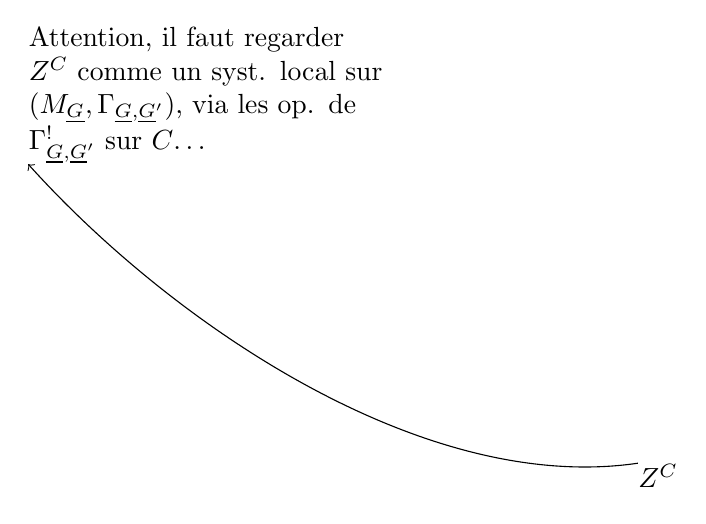
\begin{tikzpicture}[x=1cm,y=1cm]
\node[anchor=base,inner sep=0pt] (z80) at (8,0) {$\mathbb Z^C$};
\node[anchor=south west,align=left,text width=5cm,inner sep=0pt] (attention80) at (0,4.1) {Attention, il faut regarder $\mathbb Z^C$ comme un syst. local sur $(M_{\underline G},\Gamma_{\underline G,\underline G'})$, via les op. de $\Gamma^!_{\underline G,\underline G'}$ sur $C$\ldots};
\draw[->] (z80.north west) .. controls (5,-0.1) and (1.8,2.1) .. (attention80.south west);
\end{tikzpicture}}
, où $C$, on le rappelle, est l'ens. des \deleted{\unsure{flèches|frontières}}\inserted{arêtes} de $\underline G$
\margin{\uline{NB} $(M_G\deleted{,\unsure{\Gamma_{\underline G,\underline G'}}})$ est un $K(\pi,1)$, et par conséquent dans la suite exacte des $\pi_1$ de la fibration qui précède \unsure{incluse}, on a bien un $1$ à gauche}
\margin{79}

\scanpage{81}
qu'on a contracté pour former la générisation $\underline G'$. \deleted{\unsure{Plus}} (On reviendra sur la structure de cette extension, comme un produit fibré d'extensions, un peu plus bas\ldots) L'hom $\gamma_{\underline G\unsure{{}^*|{}'},\underline G'}$ s'appelle \uline{l'hom de générisation} \unsure{\uline{sur}|sur} \uline{les groupoïdes fondamentaux}, associé à l'hom de générisation $\underline G\to\underline G'$.

On va dégager une propriété de transitivité sur ces homs de générisation, pour un composé d'hom\unsure{s} de générisation
\[
\tag{104}
\diagram{\begin{tikzcd}[ampersand replacement=\&]
\underline G \arrow[r] \& \underline G' \arrow[r] \& \underline G''
\end{tikzcd}}
\]
qui donne naissance à un diagramme de groupoïdes
\deleted{\[
\diagram{\begin{tikzcd}[ampersand replacement=\&, row sep=large,column sep=large]
\Pi\unsure{M^*_{\underline G,\underline G'}|M_{\underline G^*,\underline G'}} \arrow[r] \arrow[d] \& {} \\
\Pi M_{\underline G}
\end{tikzcd}}
\]}
\margin{80}

\scanpage{82}
\mspage{(40)}
\[
\tag{105}
\diagram{\begin{tikzcd}[ampersand replacement=\&, column sep=small,row sep=large]
\Pi M^*_{G,\deleted{\unsure{G',}}G''}
 \arrow[rr,dashed,"\text{(2 cart)}"'] \arrow[d,dashed]
 \arrow[dd,bend right=35,"\varphi_{G,\unsure{G''}}"']
 \arrow[rrr,bend left=22,"\gamma_{G,G''}","\rightarrow"{pos=.80,sloped,inner sep=0pt}]
\&\& \Pi M^*_{G',G''} \arrow[r,"\gamma_{G',G''}"] \arrow[d] \& \Pi M_{G''} \\
\Pi M^*_{\underline G,\underline G'} \arrow[r,"\gamma_{G,G'}"] \arrow[d]
\& \deleted{\Pi M_{\underline{\unsure{G'}}}} \arrow[r,"\deleted{\mathrm{can}}","/\!/\!/"{pos=.5,sloped,inner sep=0pt}]
\& \begin{gathered}\Pi M_{G'\deleted{,\unsure{G''}}}\\(\simeq\Pi(M_{G'},\Gamma^!_{G',G''})\end{gathered}
\& \text{(103) pour }(G',G'')\\
\Pi M_{G,\deleted{\unsure{G'}}} \& \text{(103)} \\
\deleted{\unsure{(\simeq\Pi M)}}
\arrow[phantom,from=2-2,to=3-1,"\Bigg\}"{rotate=-48,inner sep=0pt}]
\arrow[phantom,from=1-4,to=2-3,"\Bigg\}"{rotate=-48,inner sep=0pt}]
\end{tikzcd}}
\]
\margin{\figure{\begin{tikzpicture}[x=1cm,y=1cm]\draw[line width=.2pt] (0,.02)--(.24,0);\draw[line width=.8pt] (.47,-.02)--(.56,-.02);\end{tikzpicture}}}

Dans ce diagramme, on a \deleted{\unsure{enlevé|oublié}} laissé tomber les soulignés pour les MD-graphes, \deleted{et \unsure{on a} remplacé la notation $\Pi(M_{G,G'},\Gamma^!_{G,G'})$ par la notation plus légère $\Pi M_{G,G'}$, de $=$ pour $\Pi M_{G',G''}$.} On \deleted{\unsure{tire} de (105)}\inserted{\deleted{\unsure{a défini}}} \inserted{retrouve}
\[
\tag{106}
\Pi M^*_{G,G''\deleted{\unsure{,G''|,G'}}}
\]
dans (105) comme un produit 2-cartésien --- c'est donc un groupoïde connexe, ext. de $\Pi M^*_{G,G'}$ par un $\mathbb Z^{C'}$ (tordu), et il se trouve que c'est aussi, en tant qu'ext. de $\Pi M_{G\deleted{\unsure{,G'}}}$ (de noyau une ext. de $\mathbb Z^C$ tordu par $\mathbb Z^{C'}$ tordu) une extension de $\Pi M_{G\deleted{\unsure{,G'}}}$ par un $\mathbb Z^{C\amalg C'}$ tordu\unsure{.}

De façon plus précise, on retire de (105) \uline{le} diagramme
\[
\tag{107}
\diagram{\begin{tikzcd}[ampersand replacement=\&, column sep=large,row sep=large]
\Pi M^*_{G,\deleted{\unsure{G',}}G''} \arrow[r,"\gamma_{G,\deleted{\unsure{G',}}G''}"] \arrow[d,dash,"\varphi_{G,G''\deleted{\unsure{,G'}}}","\unsure{\downarrow|\vert}"{pos=1,inner sep=0pt}] \& \Pi M_{G''} \\
\Pi M_{G\deleted{\unsure{,G'}}}
\end{tikzcd}}
\]
\margin{81}

\scanpage{85}
\[
\tag{113}
S_A\Pi M_G\overset{\mathrm{def}}=\Pi M^*_{G,G'},
\]
\margin{ici $A$ désigne l'ens de ttes les arêtes de $G$.}
\unsure{$\ast$} c'est donc une extension de $\Pi M_{G,G'}$
\margin{\figure{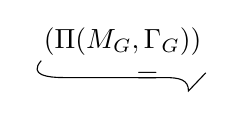
\begin{tikzpicture}[x=.55cm,y=.55cm]
\node[anchor=south west,inner sep=0] at (0,.25) {$\deleted{(\Pi\unsure{(}M_G,\unsure{\Gamma_G})\unsure{)}}$};
\node[anchor=north,inner sep=0] at (2.4,-.12) {$=$};
\draw (-.05,.14) .. controls (-.35,-.20) and (.12,-.25) .. (.45,-.25) -- (2.8,-.25) .. controls (3.15,-.25) and (3.35,-.30) .. (3.35,-.56) -- (3.75,-.14);
\end{tikzpicture}}}
par $\mathbb Z^{A(G)}$ \inserted{\deleted{d\unsure{e}}}, où $A(G)$ est l'ens. des arêtes de $G$.

Bien entendu, le groupe $\Gamma=\operatorname{Aut}G$ opère non seulement sur $M_G$ et sur $\Pi M_G$, mais aussi sur $S_A\Pi M_G$ \deleted{$=\unsure{\Gamma|F}$} (via son action sur $M^*_{G,G'}$), de façon à commuter au morphisme canonique
\[
\tag{114}
\diagram{\begin{tikzcd}[ampersand replacement=\&]
S_A\Pi M_G \arrow[r] \& (\Pi M_G,\deleted{\unsure{\Gamma}}_G)
\end{tikzcd}}
\]
ce qui permet, pour $\forall$ sous-groupe \deleted{$\Gamma'$}
\[
\Gamma'\subset\Gamma_G
\]
de définir une extension
\margin{\figure{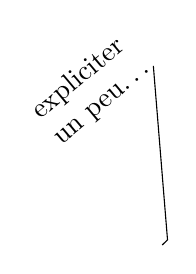
\begin{tikzpicture}[x=.45cm,y=.65cm]
\node[anchor=south west,rotate=40,align=left,inner sep=0] at (0,1.75) {expliciter\\un peu\ldots};
\draw (2.5,3.4) -- (2.9,0) -- (2.75,-.10);
\end{tikzpicture}}}
\[
\tag{115}
\diagram{\begin{tikzcd}[ampersand replacement=\&,column sep=small,row sep=small]
(S_A\Pi M_G,\Gamma') \arrow[rr] \& {} \& (\Pi M_G,\inserted{\Gamma'}\deleted{\unsure{\Gamma_G}})\\
\text{ou } S_A\Pi(M_G,\Gamma') \& \unsure{\text{ou}|{-}|\to} \& \Pi(M_G,\Gamma')
\end{tikzcd}}
\]
\deleted{\unsure{Soit} $C$ un ensemble d}
\inserted{dont le ``noyau'' est le système local} $\mathbb Z^{A(G)}$ sur $(\Pi M_G,\Gamma')$, tordu grâce à l'action de $\Gamma'$ sur $A(G)$. Si $C\subset A(G)$ est stable par l'action de $\Gamma'$, alors on a un hom
\[
\tag{116}
\diagram{\begin{tikzcd}[ampersand replacement=\&]
\mathbb Z^{A(G)} \arrow[r] \& \mathbb Z^C
\end{tikzcd}}
\]
\margin{84}

\scanpage{86}
\mspage{42}
de systèmes locaux, qui permet de construire une extension quotient de $(S\Pi M_G,\Gamma')$, extension du groupoïde $(\Pi M_G,\Gamma')$ par $\mathbb Z^C$, qu'on va noter
\[
\tag{117}
(S_C\Pi M_G,\Gamma').
\]
\deleted{Dans le cas où $\Gamma'=\Gamma^!_{G,G'}$, avec $G'=G/C$, on retrouve l'extension $\Pi M^*_{G,G'}$ de $\Pi M_{G,G'}$ par $\mathbb Z^C$ (tordu).}
\[
\tag*{\deleted{(118}}
\deleted{(S_C M_G,\Gamma_{G,G/C})\simeq\Pi M^*_{G,G/C}}
\]

On va plutôt expliciter les données en termes de
\[
\diagram{\begin{tikzcd}[ampersand replacement=\&]
S_A\Pi M_G \arrow[r] \& (\Pi M_G,\Gamma_G^!)
\end{tikzcd}}
\]
Si $G'\inserted{\simeq G/C}$ est une \deleted{\unsure{spécialisation}}\inserted{générisation} de $G$, alors on a
\[
\tag{11\deleted{\unsure{8}}9}
\diagram{\begin{tikzcd}[ampersand replacement=\&]
S_A\Pi M_G \arrow[r] \& S_{A'}\Pi M_{G'}
\end{tikzcd}}
\]
qui passe aux quotients en
\[
\tag{1\deleted{\unsure{19}}20}
\diagram{\begin{tikzcd}[ampersand replacement=\&, column sep=large,row sep=large]
S_{\inserted{A}}\deleted{A}\Pi M_G \arrow[r,dash,"\gamma_{G,G'}","\unsure{\rightharpoondown|{-}}"'{pos=.92,sloped,inner sep=0pt}] \arrow[d] \& S_{A'}\Pi M_{G'} \arrow[d] \\
S_C\Pi M_G\deleted{\unsure{\Gamma}^!} \arrow[r] \& \Pi M_{G'}
\end{tikzcd}}
\]
compatible avec l'action de $\Gamma_{G,G'}$, donc \deleted{\unsure{que}} la deuxième flèche horizontale \unsure{:|à} son tour
\margin{85}

\scanpage{87}
\unsure{se|de} factorise en
\[
\tag{121}
\diagram{\begin{tikzcd}[ampersand replacement=\&, column sep=large]
\underbrace{(S_C\Pi M_G,\Gamma^!_{G,G'}\unsure{\deleted{\prime}|{}_{h}})}_{\deleted{\Pi M^*_{G,\unsure{G'}}}} \arrow[r] \& \Pi M_{G'},
\end{tikzcd}}
\]
\deleted{\unsure{que}}\inserted{et} plus \unsure{général\textsuperscript{t}|généralement}, si $\Gamma^!_{G,G'}\subset\Gamma'\subset\Gamma_{G,G'}$ est un sous-groupe de $\Gamma=\operatorname{Aut}G$ qui stabilise $C$ et contient $\Gamma^!_{G,G'}$, on trouve
\[
\tag{122}
\diagram{\begin{tikzcd}[ampersand replacement=\&, column sep=large,row sep=large]
(S_S\Pi M_G,\Gamma') \arrow[r] \arrow[d,phantom,sloped,"\simeq"] \& (\Pi M_{G'},\Gamma'/\Gamma^!_{G,G'}).\\
(\Pi M_{G,G'},\Gamma'/\Gamma^!_{G,G'})
\end{tikzcd}}
\]

Ici la relation de transitivité un peu compliquée \inserted{(10\unsure{5|6})} s'exprime, plus simplement, par le fait que les \inserted{\unsure{groupoïdes}} $S_A\Pi M_G$ dépend fonctoriellement des \inserted{MD-}graphes $G$, pour les morphismes de générisation.

On va axiomatiser un peu. \deleted{plus}. MD-graphes \inserted{et morphismes de générisation} forment une \tikz[baseline=(cat87.base)]{\node[inner sep=0pt] (cat87) {catégorie};\draw[->] (cat87.south west)--(cat87.south east);}, $(\deleted{\unsure{\mathcal G}}\mathfrak g)$, où tous les morphismes sont des épimorphismes. Cette catégorie satisfait
\margin{La catégorie $\mathcal G$ joue le rôle d'un ens. de \unsure{complexes|complexités|``types''} \unsure{géométriques} ou des cas..}
\margin{86}

\scanpage{88}
\mspage{43}
à la condition suivante

(123) (Simp) Pour $\forall\ G\in\mathcal M$, l'ens ordonné des quotients \inserted{$G'$} de $G$ est \deleted{\unsure{isomorphe} à un \unsure{simplexe}}\inserted{un ``simplexe'' i.e. isomorphe} à l'ens des parties d'un ens fini.

Si $A_G$ désigne l'ens des quotients de $G$ qui sont $\ne G$ et qui sont \deleted{\unsure{minimaux|maximaux}}\inserted{\unsure{maximaux|minimaux}} parmi ceux-ci, alors l'ens \inserted{ordonné} des quotients de $G$ est donc isomorphe à l'ens des parties de $A_G$. \deleted{Si} On désigne par $G/C$ le quotient de $G$ associé à $A_G\setminus C$ (d'autant plus petit que $C$ est plus grand)\unsure{.}

\margin{\uline{NB} Il faudrait montrer comment cette axiomatisation s'applique à $\forall$ situation de multiplicités, \deleted{\unsure{topologiques ou étales|topologiques ordinaires}}\inserted{analytiques relatives} avec un diviseur à croisements normaux.... (à cela près que $S\Pi M_G$ est une extension de $\Pi M_G$ non pas par un $\mathbb Z^C$ tordu, mais par un quotient d'un tel.\unsure{-|..}}

On suppose donné pour $\forall\ G\in\operatorname{Ob}\mathcal G$ deux groupoïdes $S\Pi M_G$ et $\Pi M_G$, et un morphisme
\[
\tag{124}
\diagram{\begin{tikzcd}[ampersand replacement=\&,column sep=1em]
S\Pi M_G \& \overset{\varphi_G}{\unsure{\rightharpoondown|{-}}} \& \Pi M_G.
\end{tikzcd}}
\]
On suppose que $\varphi_G$ fait de $S\Pi M_G$ une extension de $\Pi M_G$ par $\mathbb Z^{A(G)}$. (en fait, c'est une structure supplémentaire sur $S\Pi M_G$). On suppose que $G\mapsto\Pi M_G$ est un foncteur en $G$ \uuline{pour les iso} (pas pour les morphismes quelc.)
\margin{87}

\scanpage{89}
et que $\inserted{G\mapsto}S\Pi M_G$ est un foncteur en \deleted{$\unsure{M}_G$} $G$ pour les morphismes quelconques, et que (124) est fonctoriel pour les iso. Pour un morphisme quelconque $G\xrightarrow{f}G'$, correspondant à une partie $C\subset A_G$ (telle que $G\unsure{\rightharpoondown|{-}}G'$ soit isom, en tant que quotient de $G$, à $G\unsure{\rightharpoondown|{-}}G/C$), on suppose que l'on a un diagramme commutatif
\[
\tag{125}
\diagram{\begin{tikzcd}[ampersand replacement=\&, column sep=large,row sep=large]
S\Pi M_G \arrow[r,"S\Pi(f)"] \arrow[d,"\varphi_G"] \& S\Pi M_{G'} \arrow[d,"\varphi_{G'}"] \\
S_{\deleted{\unsure{A}}C}M_G \arrow[r,"\gamma_f"] \& \deleted{\unsure{S}}\Pi M_{G'}
\end{tikzcd}}
\]
i.e. que le composé
\[
\diagram{\begin{tikzcd}[ampersand replacement=\&, column sep=large]
S\Pi M_G \arrow[r,"S\Pi(f)"] \& S\Pi M_{G'} \arrow[r,phantom,"{\overset{\varphi_{G'}}{\unsure{\rightharpoondown|{-}}}}" description] \& \Pi M_{G'}
\end{tikzcd}}
\]
se factorise par l'extension $S_{\deleted{\unsure{A}}C}M_G$ de $\Pi M_G$ par $\mathbb Z^C$, déduite de l'extension $S\Pi M_G$ de $\Pi M_G$ par $\mathbb Z^{A(G)}$ grâce à l'hom canonique
\[
\diagram{\begin{tikzcd}[ampersand replacement=\&]
\mathbb Z^{A(G)} \arrow[r] \& \mathbb Z^C.
\end{tikzcd}}
\]
On a automatique alors la relation de transitivité pour un composé.
\margin{88}

\scanpage{90}
\mspage{44}
10) \uline{Structure} MDT \uline{discrète} : \uline{action} des \uline{morphismes de normalisation entre \inserted{MD-}graphes}

Nous voulons exprimer, en plus des morphismes
\deleted{\inserted{$\varphi_{\unsure{G}}$ \unsure{et}}}
$S\Pi f$ ($f$ morphisme de générisation) et $\Pi f$ ($f$ iso de MD-graphes)
entre autres des morphismes du type
\diagram{\begin{tikzcd}[ampersand replacement=\&]
M_G \arrow[r] \& M_{g_\alpha,\widehat I_\alpha}
\end{tikzcd}}
\diagram{\begin{tikzcd}[ampersand replacement=\&,column sep=large]
\text{\unsure{etc|et}} \& M^{?}_{g,\unsure{I|\overline I}} \arrow[r] \& M_{g,I'} \& \text{pour }I'\subset I.
\end{tikzcd}}
On va introduire pour ceci une autre notion de morphismes de MD-graphes,
qu'on appellera morphismes de normalis\unsure{at}
(l'intersection des deux notions de morphisme est celle d'iso de MD-graphes).

Géométriquement, cela correspondra à la situation d'une courbe stable
\deleted{$(\widehat X,\unsure{I)}$}\inserted{$X=\widehat X\setminus I$}
sur un corps alg. clos $\unsure{h|k}$, en distinguant une partie $I'\subset I$
de l'ens des pts à l'infini, et une partie $A'\subset A$ de l'ens des pts doubles de $X$,
\margin{89}

\scanpage{92}
\mspage{45}
complet de $X'$ se déduit de celle de $X$, en prenant la $=$ application genre, et $I'\longrightarrow S$ induit par $I\longrightarrow S$.

En fait, quand on a normalisé $\widehat X$ en les pts de $A^{\unsure{a|e|2}}\setminus A'$ pour obtenir $\widehat X'$, on a sur $\widehat X'$, en plus des pts marqués indexés par $I$ et des pts \deleted{\unsure{quadratiques|quadruples}}\inserted{doubles} indexés par $A'$, un troisième ens. remarquable de ``pts marqués'', savoir l'image inverse \inserted{$\widetilde J$} de $J=A\setminus A'$, \deleted{\unsure{E|En}} de cardinal égal à $2\operatorname{Card}(A\setminus A')$. En termes de la courbe normale propre $Y$ \deleted{\unsure{qui}} contenant $\widetilde A\amalg I$, qui définit $\widehat X$ comme $Y/\sigma_{\widetilde A}$ et $X$ comme $(Y\setminus I)/\sigma_{\widetilde A}$, $\widehat X'$ est défini comme $Y/\sigma_{\widetilde A'}$, ce qui nous donne un ens. de pts marqués lisses \deleted{$\unsure{A}$} $\widetilde J\amalg I$ sur $\widehat X'$. Ceci étant, au lieu d'``oublier'' $\widetilde J$ et $I\setminus I'$ pour ne retenir que l'ens de pts marqués
\margin{91}

\scanpage{93}
$I'$ sur $\widehat X'$, on peut aussi, plus généralement, se donner une partie $I'$ (non pas de $I$, mais de) $\widetilde J\amalg I$, qu'on retiendra comme ``pts marqués''.

Quand on s'est ainsi donné (pour \unsure{un|une} \deleted{\unsure{MD}}m\unsure{.}graphe $\underline G$ donné) une partie $A'$ de $A(G)$, et une partie $I'$ de $I\amalg\widetilde J$ (où $\widetilde J=\widetilde A(G)-\widetilde A'\deleted{\unsure{)}}$, alors pour $\forall$ courbe spéciale $G$-épinglée, on déduit une courbe spéciale, qui sera épinglée par le m\unsure{.}graphe $\underline G'$ déduit de $\underline G,A',I'$ en prenant le \unsure{ss|s|sous|x}-graphe \inserted{$G'$ de $G$} ayant $=$ $S$ sommets, et ayant $A'$ comme ens. d'arêtes, \unsure{avec|on} comme ``ens de pts marqués'' $I'\subset I\amalg\widetilde J$, qui s'envoie dans $S$ \deleted{\unsure{s}i} par
\[
(126)\qquad I'\longrightarrow S\quad\text{induit par }I\longrightarrow S\text{ et }\widetilde A(G)\xrightarrow{\text{origine}}S,
\]
l'application genre pour $\underline G'$ est celle pour $\underline G$.
\margin{92}

\scanpage{94}
\mspage{46}
On peut généraliser encore un peu ces construction\unsure{s}, en \deleted{\unsure{choisissant} une \unsure{partie}} \inserted{remplaçant $X'$ par} \inserted{une réunion de composantes connexes} \deleted{de \unsure{composantes} \unsure{irréductibles}}, contenant $A'$ et $I'$. Cela revient à prendre un sous-graphe \uline{quelconque} $G'$ de $G$ (n'ayant pas $\text{néc.}^{\text{t}}$ \deleted{les} $=$ ens. de sommets, mais un ens. de sommets $S'\subset S$), [défini donc par la donnée d'une partie $S'$ de $S$, d'une partie $\widetilde A'$ de $\widetilde A(G)$ st.ble par $\sigma_{\widetilde A}$ et telle que $o_G:\widetilde A\unsure{\rightharpoonup|{-}}S$ applique $\widetilde A'$ dans $S'$], plus une partie $I'$ de $I\amalg\deleted{\unsure{\widetilde A}}\widetilde J$ (où $\widetilde J=\widetilde A\setminus\widetilde A'$), appliquée dans $\underline{S}'$ par l'\deleted{\unsure{application origine}}\inserted{application}
\[
\begin{aligned}
I\amalg\widetilde J\longrightarrow S\quad &\text{induit par }I\longrightarrow S\\
&\text{et par }\widetilde A\xrightarrow{o_G}S.
\end{aligned}
\]

Un cas particulièrement important est celui où $G'$ est un sous-graphe ponctuel, défini par un $\alpha\in S$, \inserted{donc $\widetilde J=\unsure{\widetilde A|A}$,} et où on prend
\[
\begin{gathered}
I'=I_\alpha\amalg\widetilde A_\alpha=\text{image inverse de }\{\alpha\}\text{ par}\\
I\amalg\widetilde A\longrightarrow S.
\end{gathered}
\]

Si on veut exprimer ces constructions en termes d'une notion ad-hoc de
\margin{93}

\scanpage{95}
``morphisme'' (de normalisation) de m.graphes, on aboutit à la

\uline{Définition} Soient $\underline G=(\underbrace{S,\widetilde A,\sigma_{\widetilde A},o_G}_{G},I\longrightarrow S\overset{\underline g}{\unsure{-|\longrightarrow}}\mathbb N)$ et $\underline G'=(\underbrace{S',\ldots}_{G'})$ deux m\unsure{.}graphes. On appelle \uline{morphisme de \deleted{\inserted{\unsure{pré}}}normalisation} de $\underline G'$ dans $\underline G$ la donnée d'un couple \deleted{$\unsure{f_G}$ \unsure{de}} $(f_G,f_I)$, où

a) $f_G:G'\unsure{\rightharpoondown|\longrightarrow}G$ est un hom de graphes, qui est injectif sur les sommets et injectif sur l'ens des arêtes (donc identifie $G'$ à un sous-graphe de $G$)

\margin{On suppose de plus c) $\forall s'\in S',\quad \underline g^{\unsure{\prime\prime|\prime}}(s')=\underline g(f_G(s'))$}

b) $f_I:I'\longrightarrow I\amalg\widetilde A\deleted{(\unsure{G})}$ est une application injective, dont l'image est contenue $I\amalg\widetilde J$, \unsure{avec|où} $\widetilde J=\widetilde A(G)\setminus f_{\unsure{G'|G}}(\widetilde A'\deleted{\unsure{(G'}})$ et rendant commutatif le diagramme
\diagram{(129)\qquad\begin{tikzcd}[ampersand replacement=\&,row sep=small,column sep=large]
I' \arrow[r,hook] \arrow[d] \& I\amalg\unsure{A|\widetilde A} \arrow[d] \\
S' \arrow[r,hook,"\unsure{\forall}" description] \& S
\end{tikzcd}}
\margin{On dit que $f$ est un \uline{morphisme de normalisation strict} si $S'\xrightarrow{\sim}S$, et si $I'\simeq I\amalg\widetilde J$.}

Par exple, iso. de m.graphes est un morphisme de normalisation. \deleted{\unsure{On}}

Voici une façon de raccorder cette notion à une notion ``orthodoxe'' de morphismes de graphes, en mettant ``dans un même sac'', pour un m.graphe
\margin{9\unsure{4|5}}

\scanpage{96}
\mspage{47}
donnée $G$, l'ens $\widetilde A(G)$ et $I(G)$ (munis l'un et autre d'une application \inserted{``origine''} à valeurs dans $S(G)$).

Pour ceci, on \unsure{a|à|va} utiliser la notion de ``graphes avec branches aplaties'', qui généralis\unsure{e} celle de graphe, et topologiquement correspond à la classification des \unsure{\deleted{4}|4|\deleted{q}|q} couples $(X,S)$ d'un espace topologique compact $X$, et d'une partie finie $S$, tels que a) $X$ soit une étoile \unsure{au|en} voisinage de $\forall$ pt de $S$, \deleted{\unsure{et|a}} b) \deleted{\unsure{S}} tt composante connexe de $X\setminus S$ est une $1$-variété à bord non compacte (car on veut que tout \deleted{\unsure{adhérence} d'} ``arête'' ait un sommet). \unsure{Il|Ça} revient au $=$ de dire que $X$ est un $1$-complexe top, et $S$ une partie finie qui contient les sommets d'ordre $\geq3$, et telle qu'aucune composante connexe de $X\setminus S$ ne soit compacte (i.e. que tt composante connexe de $X$ contienne un sommet, i.e. $S\unsure{\rightharpoondown|{-}}\unsure{\Pi|\pi}_0(X)$ est surjectif).

Ceci se classifie combinatoirement par des systèmes $(S,\unsure{\widehat A|\widehat I},\sigma_{\unsure{\widehat A|\widehat I}},o_{\widetilde A})$, où \deleted{$\unsure{\widetilde A=\sigma_{\widetilde A}|\widetilde A,\sigma_A|\widetilde A,o_A}$} $S,\unsure{\widehat A|\widehat I}$ sont des ens finis, $\sigma_{\unsure{\widetilde A|\widehat A}}$ est une involution de $\widetilde A$, et $o_{\widetilde A}:\widetilde A\unsure{\rightharpoondown|{-}}S$ une
\margin{95}

\scanpage{97}
application. On n'exige plus que $\sigma_{\unsure{\widehat I|\widehat A}}$ soit sans pts fixes — l'ens des pts fixes, $I$, \deleted{\unsure{se|de}} correspond aux ``branches aplaties'' du \inserted{$1$-}complexe i.e. aux \deleted{``\unsure{bouts}''} ``pts-bord'' de $X$ qui ne sont pas dans $S$. La donnée d'un graphe à branches aplaties revient donc (en décomposant $\widehat I$ en $I\amalg\widetilde A$, où $I=\widehat I^\sigma$ et $\widetilde A=\widehat I\setminus\unsure{\widehat I^\sigma|I}$) à la donnée d'un \deleted{\unsure{couple}} graphe ordinaire \inserted{$(S,\widetilde A,\sigma_{\widetilde A},o_{\widetilde A})$}, plus un ensemble $I$ et une application $I\longrightarrow S$.

On décrit un tel graphe à branches aplaties par un graphisme tel que
\figure{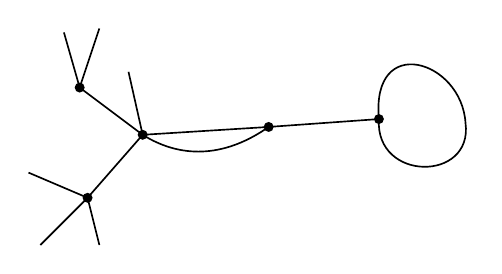
\begin{tikzpicture}[x=1cm,y=1cm,line width=.6pt]
\coordinate (a) at (0,0); \coordinate (b) at (-.8,.6); \coordinate (c) at (-.7,-.8); \coordinate (d) at (1.6,.1); \coordinate (e) at (3,.2);
\draw (a)--(b) (a)--(c) (a)--(d)--(e);
\draw (a) to[out=-32,in=-145] (d);
\draw (e) .. controls (2.9,1.3) and (4.05,.95) .. (4.1,.15) .. controls (4.2,-.6) and (2.95,-.6) .. (e);
\draw (b)--(-1,1.3) (b)--(-.55,1.35) (c)--(-1.45,-.48) (c)--(-1.3,-1.4) (c)--(-.55,-1.4) (a)--(-.18,.8);
\foreach \p in {a,b,c,d,e} {\fill (\p) circle (1.8pt);}
\end{tikzpicture}}
où les sommets sont figurés par des points ``gros $\bullet$, et les branches aplaties \deleted{sont} se distinguent par le fait justement qu'elles ne sont pas marquées \inserted{en} gros. Le graphe \inserted{à b.a.} ci-dessus correspond donc, avec la notion des ``pieds marqués'', à
\figure{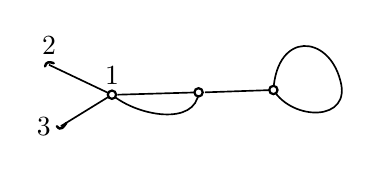
\begin{tikzpicture}[x=1cm,y=1cm,line width=.6pt]
\coordinate (a) at (0,0); \coordinate (b) at (-.8,.38); \coordinate (c) at (-.65,-.4); \coordinate (d) at (1.1,.03); \coordinate (e) at (2.05,.06);
\draw (b)--(a)--(c);
\draw (.07,0)--(d) (1.18,.03)--(e);
\draw (a) to[out=-40,in=-95] (d);
\draw (e) .. controls (2.1,.81) and (2.75,.76) .. (2.9,.18) .. controls (3.05,-.34) and (2.3,-.34) .. (e);
\draw[line width=.9pt,line cap=round] (-.85,.36) .. controls (-.84,.42) and (-.79,.42) .. (-.74,.40);
\draw[line width=.9pt,line cap=round] (-.70,-.40) .. controls (-.65,-.47) and (-.61,-.40) .. (-.58,-.36);
\foreach \p in {a,d,e} {\draw[fill=white,line width=.8pt] (\p) circle (1.5pt);}
\node[above] at (a) {$1$}; \node[above] at (b) {$2$}; \node[left] at (c) {$3$};
\end{tikzpicture}}
\margin{96}

\scanpage{98}
\mspage{48}
\margin{Cas d'un morphisme de normalisation strict.}
Dans cette optique, on voit que dans le cas où \inserted{$S'\simeq S$,} $I'\xrightarrow{\sim}I\amalg\widetilde J$, on obtient $G'$ à partir de $G\deleted{\unsure{'}}$ en se donnant l'ens. $C$ de \deleted{\unsure{flèches|pieds}}\inserted{arêtes (ordinaires)} de $G\deleted{\unsure{'}}$ ``qu'on veut enlever'' (\inserted{$\widetilde C$ est le} complémentaire de $I'$ ds $(\widehat I'\longrightarrow\widehat I)$ en prenant un pt sur chaque arête $\in C$, et en ``coupant'' l'arête en ce point avec un coup de ciseaux (i.e prenant la découpe de $X$ suivant la partie finie marquée sur $X$)

% Two opening parentheses precede the complement expression, but only one closing parenthesis is visible there.
\figure{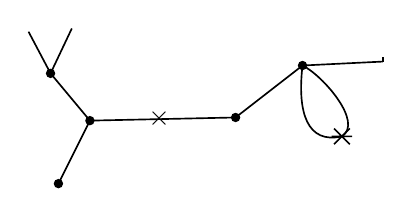
\begin{tikzpicture}[x=1cm,y=1cm,line width=.6pt]
\coordinate (a) at (0,0);
\coordinate (b) at (-.5,.6);
\coordinate (c) at (-.4,-.8);
\coordinate (d) at (1.85,.04);
\coordinate (e) at (2.7,.7);
\draw (b)--(a)--(c) (a)--(d)--(e);
\draw (b)--(-.78,1.13) (b)--(-.23,1.17) (e)--(3.72,.75);
\draw (3.72,.75)--(3.72,.81);
\draw (e) .. controls (2.63,.1) and (2.76,-.3) .. (3.2,-.2)
  .. controls (3.48,-.02) and (2.95,.58) .. (e);
\foreach \p in {a,b,c,d,e} {\fill (\p) circle (1.7pt);}
\node at (.88,.02) {$\times$};
\draw (3.10,-.30)--(3.30,-.10) (3.10,-.10)--(3.30,-.30) (3.07,-.2)--(3.33,-.2);
\end{tikzpicture}}
donne
\figure{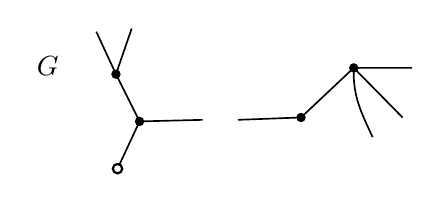
\begin{tikzpicture}[x=1cm,y=1cm,line width=.6pt]
\node[left] at (-.9,.7) {$G$};
\coordinate (a) at (0,0);
\coordinate (b) at (-.3,.6);
\coordinate (c) at (-.28,-.6);
\coordinate (d) at (2.05,.05);
\coordinate (e) at (2.72,.68);
\draw (b)--(a)--(c) (a)--(.8,.02) (b)--(-.55,1.14) (b)--(-.1,1.18);
\draw (1.25,.02)--(d)--(e) (e)--(3.46,.68) (e)--(3.34,.05);
\draw (e) to[out=-92,in=115] (2.96,-.2);
\foreach \p in {a,b,d,e} {\fill (\p) circle (1.7pt);}
% The lower-left endpoint has a visible open centre in this drawing.
\draw[line width=.8pt,fill=white] (c) circle (1.7pt);
\end{tikzpicture}}

On trouve un nouveau graphe à branches aplaties (qui a des chances d'être disconnexe, $\overline{m}$ si $G$ était connexe \unsure{\}|!} — $=$ si $G$ n'avait pas de branches aplaties, il a tendance à en avoir\ldots).
\margin{En sens inverse, se déduit de $G'$ en se donnant une involution ss pts fixes \unsure{dans|de} l'ens de ses branches ``aplaties'', ce qui permet de ``recoller'' celles-ci par leurs bouts.}
Si de plus on \deleted{\unsure{f}} remplace $G'$ par un sous-graphe déduit de $G'$ en enlevant certaines branches aplaties, et en prenant une réunion de composantes connexes de ce qui reste (en \deleted{\unsure{préservant|inversement})} \inserted{en outre} c'est
% The baseline en survives; the raised en is separate. The old closing parenthesis is crossed out.
\margin{97}

\scanpage{99}
kif-kif, car les composantes connexes ne changent pas en ajoutant ou retranchant des branches aplaties), on trouve la relation la plus générale entre $G$ et un $G'_0$, du type explicité dans la définition. des ``morphismes de normalisation de m.graphes''.

On définit de façon évidente les composés de morphismes de normalisation. Le composé de morphismes de \unsure{normalisat} strict est strict. Les m.graphes avec morphismes de normalisation strict font une catégorie, dont les iso. sont les iso. ordinaires de m.graphes. Les morphismes de cette catégorie sont des monomorphismes. Quand on se borne aux morphismes \inserted{de norm.} stricts, on voit que (comme pour les morphismes de générisation) l'ens des sous-m.graphes stricts d'un m.graphe \inserted{$G$} est un ens. ordonné \deleted{\unsure{iso}}\inserted{anti}morphe à l'ens des parties de $A(G)$, en associant à tte partie $C\subset A(\unsure{G|C})$
\margin{98}

\scanpage{100}
\mspage{49}
la ``\uline{découpe}'' de $G$ suivant $C$, obtenue en ``coupant'' comme il a été dit les les milieux des arêtes $\in C$ (ce qui revient à ``enlever'' les arêtes, et à remplacer les côtés correspondants par des pts marqués.)

Soit un morphisme de normalisation entre m\unsure{.}graphes
\[
(130)\qquad G'\longrightarrow G\deleted{\unsure{'}}
\]
Si c'est un morphisme de normalisation \uline{strict}, on voit que $G'$ est stable ssi $G$ l'est. (Dans le cas général, on voit que si $S'\unsure{-|\rightharpoondown}S$ est surjectif, et si $G'$ est stable, $G$, l'est aussi)

\deleted{\unsure{Supp.}} Si $X$ est une courbe spéciale (sur une base quelconque $S$), épinglée par $G$, alors on voit (en procédant comme au début de la section) qu'on lui associe canoniquement une courbe spéciale $\unsure{C|G}'$ épinglée, d'où un foncteur
\[
(13\unsure{0|1})\qquad M_G(S)\longrightarrow M_{G'}(S),
\]
\margin{99}

\scanpage{101}
qui pour $S$ variable est compatible \unsure{aux|avec} chgt de base, et donne donc un morphisme de multiplicités modulaires \inserted{(si $G,G'$ sont stables)}
\[
(132)\qquad M_G\longrightarrow M_{G'},
\]
avec fonctorialité évidente pour les composés. Ainsi $M_G$ est un \uline{foncteur contravariant en} $G$ pour les morphismes de normalisation \inserted{de m.graphes stables}. Cette fois, on a

\uline{Proposition} a) Si $G\longrightarrow G'$ est un morphisme de normalisation \uline{strict}, alors (132) est un \uline{iso.} de multiplicités

b) Soient $G_\alpha$ des \deleted{\unsure{composantes connexes|graphes connexes}}\inserted{m.graphes stables} \deleted{\unsure{de}} $G$ le m.graphe somme des $G_\alpha$. Alors\unsure{:|,} le morphisme
\[
(133)\qquad M_G\unsure{\rightharpoondown|{-}}\prod_\alpha, M_{G_\alpha}
\]
\unsure{est} un iso. de multiplicités.
\margin{\uline{NB} On remplace la notation $\Pi M_G$ par $\Pi_1M_G$, pour ne pas \unsure{confondre} $\Pi_1\deleted{\unsure{\Pi|M_G}}$ le signe du produit}

\uline{Cor} $\Pi_1M_G$ est un foncteur contravariant en \deleted{\unsure{le}} m.graphe stable $G_{\deleted{\unsure{\alpha|f}}}$ pour les
\margin{100}

\scanpage{102}
\mspage{50}
morphismes de normalisation — il \unsure{transf} morph. de norm. stricts en \deleted{\unsure{isomorphismes}}\inserted{équivalences} de \deleted{\unsure{multi}}groupoïdes, et sommes de m.graphes stables en produit des groupoïdes correspondants.

Pour nous, l'intérêt principal est dans la formule (obtenue en prenant le ``sous-objet strict'' minimal de $G$)
\[
(144)\qquad \Pi_1M_G\approxeq\prod_{\alpha\in S}\Pi_1M_{\unsure{g|G}_\alpha,\widehat I_\alpha)}^{\deleted{\unsure{*|\alpha|\wedge}}}
\]
qui tient compte \inserted{de} (et redonne \unsure{automatiq\textsuperscript{t}}) les \deleted{\unsure{isomorphismes}}\inserted{équivalences} des $\Pi M_{G'}\unsure{-|\rightharpoondown}\Pi M_G$ par des morphismes de norm. stricts (qui induisent en effet des iso. pour les normalisés stricts $\widetilde G'$ et $\widetilde G$ de $G$,
\diagram{\(\displaystyle (145)\qquad
\begin{tikzcd}[ampersand replacement=\&, row sep=large, column sep=large]
\widetilde G' \arrow[r] \arrow[d] \& \widetilde G \arrow[d] \\
G' \arrow[r] \& G
\end{tikzcd}
\)}
$G'\unsure{-|\rightharpoondown}G$ est un morph. de norm. strict\unsure{s} ssi le morphisme correspondant sur les normalisés (totaux) est un \uline{iso}\ldots)
\margin{101}

\scanpage{103}
Mais il faut encore expliciter la structure de $S\Pi M_G$, en termes des $M_{g_\alpha,\widehat I_\alpha}$ — nous le ferons au n° suivant.

Pour un morphisme de normalisation quelconque \unsure{(}pas. néc strict), le diagramme commutatif donne un diagramme comm (à iso de foncteurs près)
\diagram{\begin{tikzcd}[
ampersand replacement=\&, column sep=small, row sep=large,
execute at end picture={
  \node[left=2em] at (\tikzcdmatrixname-1-1.west) {$(146)$};
  \path (\tikzcdmatrixname-1-1.east) ++(.35,0) coordinate (topstart);
  \path (\tikzcdmatrixname-1-3.west) ++(-.35,0) coordinate (topfinish);
  \draw[->] (topstart) -- (topfinish |- topstart);
  \draw (topstart) -- ++(.20,-.04);
  % The short lower-left return is visible; its interpretation as a head is uncertain.
  \node[below=1pt,inner sep=0pt] at (topstart) {$\unsure{\vphantom{-}}$};
}]
\Pi_1M_{\substack{\deleted{\unsure{G'}}\\G}} \arrow[d,"\wr"]
\&\& \Pi_1M_{G'} \arrow[d,"\wr"] \\
\Pi_1M_{\widetilde G}=\prod_{\alpha\in S}M_{g_\alpha,\widehat I_\alpha}
\arrow[rr]
\arrow[dr,"{\substack{\text{on identifie }S'\\\text{à une partie de}\\S,\ \text{et }g_\alpha\text{ à }g'_{\alpha'}}}"']
\&\&
\Pi_1M_{\widetilde G'}=\prod_{\alpha'\in S'}\raisebox{-0.7ex}{\scriptsize$\deleted{\unsure{1}}$}M_{g'_{\alpha'},\widehat I'_{\unsure{\alpha'|\alpha}}} \\
\& \prod_{\alpha'\in S'}\raisebox{-0.7ex}{\scriptsize$\deleted{\unsure{*|1}}$}M_{g_\alpha,\widehat I_\alpha}
\arrow[ur,"\psi"'] \&
\end{tikzcd}}
\margin{Ceci provient d'un diagramme analogue au niveau des multiplicités modulaires elles-mêmes\ldots}

La flèche oblique $\psi$ est induite par des flèches
\[
(147)\qquad \Pi_1M_{g_\alpha,\widehat I_\alpha}\longrightarrow\Pi_1M_{g_\alpha^{\deleted{\unsure{'}}},\widehat I'_\alpha}
\]
compte tenu du fait qu'on a $\widehat I'_\alpha\subset\widehat I_\alpha$.

Ainsi la connaissance des morphismes de normalisation \inserted{généraux} est réduit à celle des morphismes
\diagram{\begin{tikzcd}[
ampersand replacement=\&, column sep=2.2em,
execute at end picture={
  \node[left=2.2em] at (\tikzcdmatrixname-1-1.west) {$(148)$};
  \path (\tikzcdmatrixname-1-1.east) ++(.12,0) coordinate (tail148);
  \path (\tikzcdmatrixname-1-2.west) ++(.31,0) coordinate (overlap148);
  \path (overlap148 |- tail148) coordinate (end148);
  \path (tail148) -- (end148) coordinate[pos=.46] (head148);
  % One continuous shaft bears two right heads; its second head crosses the target Pi.
  \draw (tail148) -- (end148);
  \draw (head148) ++(-.10,.05) -- (head148) -- ++(-.10,-.05);
  \draw (end148) ++(-.10,.05) -- (end148) -- ++(-.10,-.05);
}]
\Pi_1M_{g,I} \& \Pi_1M_{g,I'} \& \text{pour }I'\subset I,
\end{tikzcd}}
\margin{102}

\scanpage{104}
\mspage{51}
qui sont induits par les morphismes de normalisation entre m.graphes associés aux graphes \unsure{mono|uni}ponctuels. Bien entendu, pour pouvoir reconstituer bel et bien les \inserted{effets \deleted{\unsure{l'interaction}} en $\Pi_1M$ des} morphismes de normalisation, et leurs propriétés de commutation aux iso, il faut utiliser les \deleted{\unsure{covariances|commutations}} commutation de (148) à
\[
\unsure{\mathfrak S|\mathcal G}_{I,I'}\simeq\unsure{\mathfrak S|\mathcal G}_{I'}\times\unsure{\mathfrak S|\mathcal G}_{I\setminus I'}\qquad\ldots
\]

\uline{Programme} Déterminer (à équivalence ``canonique'' près) tous les groupoïdes $\Pi_1M_{g,I}$, avec leur dépendance fonctorielle pour \inserted{$g$ fixe,} $I$ variable (des mono. $I'\hookrightarrow I$) via les morphismes de normalisation (148).
\margin{par ``gén. et relations'' — \unsure{définies|définis|définir} en termes purement algébriques\ldots}

De plus, pour tt MD-graphe $G$, déterminer l'extension $S\Pi_1M_G$ de
\[
\Pi_1M_G\simeq\prod_{\alpha\in S(G)}\Pi_1M_{\alpha,\widehat I_\alpha}\quad\text{par }\mathbb Z^{\widetilde A(G)},
\]
et pour un morphisme de générisation (p.ex. un iso!) \deleted{\unsure{donné}} $G\longrightarrow G'$ de MD-graphes, \deleted{\unsure{définir}}\inserted{déterminer} le morphisme de groupoïdes de générisation correspondant
\[
S\Pi_1M_G\unsure{\longrightarrow|\rightharpoondown}S\Pi_1M_{G'}.
\]
\margin{\figure{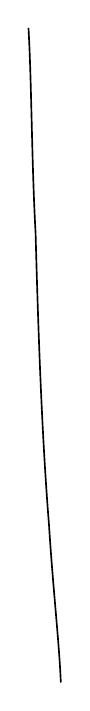
\begin{tikzpicture}[x=1cm,y=1cm]
\draw[line width=0.6pt,line cap=round] (0,0) .. controls (0.04,-0.7) and (0.04,-1.7) .. (0.09,-2.6) .. controls (0.13,-4.1) and (0.18,-5.3) .. (0.26,-6.3) .. controls (0.31,-7.1) and (0.39,-7.8) .. (0.41,-8.3);
\end{tikzpicture}}}
\margin{1\unsure{0|9}3}

\scanpage{106}
\mspage{52}
11) Digression : déployement d'un diviseur à croisements normaux.

Pour fixer les idées, je vais me placer dans le contexte des multiplicités analytiques lisses — mais on pourrait \unsure{aussi|voir}, en prenant des multiplicités analytiques lisses \uline{relatives} — ou en remplaçant l'hyp. analytique\unsure{s} par des hyp. topologiques ad-hoc — ou en passant au contexte schématique.....

Soit $X$ une multiplicité analytique lisse, et $D$ un diviseur sur $X$ à croisements normaux (hyp. purement locale en $(X,D)$, par définition). \deleted{Soit $G$ un}

Pour tout pt $x$ de $D$, l'ens des ``branches'' de $D$ passant par $x$ est un ensemble fini. $I(x)$, Par définition, les \uline{germes} \inserted{en $x$} \uline{de sous-multiplicités} \uuline{attaché\unsure{s|es}} \uuline{à $D$} sont les intersections d'un nb fini \deleted{de} parmi les $D_{x,i}\in I(x)$.
\margin{il vaut mieux prendre un $x\in X$, et poser $I(x)=\phi$ si $x\notin D$.}
Ces \unsure{germes} forment un ensemble ordonné \inserted{$\Delta_x\unsure{=(|(=}\Delta_x(X\unsure{,D}))$} antiisomorphe \unsure{à|:} $\mathcal P(I(x))$, \deleted{Si \unsure{$J$ est}}\inserted{la codimension} \deleted{\unsure{une|avec|ceux}} de $D_{x,J}$ $(J\subset I(x))$ étant donnée par
\[
(149)\qquad \operatorname{Codim}(D_{x,J},X_x)=\operatorname{card}J
\]
\margin{105}

\scanpage{107}
Soit $J$ un ensemble ordonné, on s'intéresse aux plongements d'ensembles ordonnés
\[
(150)\qquad J\mathrel{\overset{\varphi}{\hookrightarrow}}\Delta_{\unsure{x|\alpha}}\unsure{\xi}\simeq\mathcal P(I(\unsure{x|\alpha}))^\circ
\]
Un tel plongement donne une ``fonction codimension'' sur $J$, en composant, \inserted{\unsure{soit} $d$,} et \deleted{\unsure{dire} que $\varphi$ est un plongement d'\unsure{ens.} \unsure{ordonnés} signifie que}\inserted{on suppose donné déjà $d$ d'avance sur $J$} satisfaisant
\[
(151)\qquad\text{Si }x<y\quad\text{on a}\quad\unsure{d|c}(x)<c(y),
\]
et on se borne aux $\varphi$ qui sont des plongts ordonnés, compatibles aux foncts codim sur $J$ et sur $\Delta_{\unsure{x|\alpha}}$.
\deleted{On suppose de plus que $J$ \unsure{a} un plus petit élément (\unsure{ce} qui correspond donc à une codim. \unsure{maximale|minimale} \deleted{\unsure{qui est}} soit $d(J)$) — quitte à le rajouter, s'il n'y est déjà!}

Considérons, \inserted{pour tout $\unsure{q|d|p}\in\mathbb N^*$,} la multiplicité analytique formée des couples $(x,V)$, où $x$ est un pt de $D$ et $V$ un germe de sous-multi-
plicité de $X$ attaché à $D$, de codim $\unsure{q|d|p}$. On \deleted{\unsure{voit}} voit aisément que ce sont \inserted{bien} là les points d'une multiplicité analytique que je note $D_{\unsure{q|d|p}}$, et on a un morphisme
\margin{106}
